%%%%%%%%%%%%%%%%%%%%%%%%%%%%%%%%%%%%%%%%%
% Short Sectioned Assignment
% LaTeX Template
% Version 1.0 (5/5/12)
%
% This template has been downloaded from:
% http://www.LaTeXTemplates.com
%
% Original author:
% Frits Wenneker (http://www.howtotex.com)
%
% License:
% CC BY-NC-SA 3.0 (http://creativecommons.org/licenses/by-nc-sa/3.0/)
%
%%%%%%%%%%%%%%%%%%%%%%%%%%%%%%%%%%%%%%%%%

%----------------------------------------------------------------------------------------
%	PACKAGES AND OTHER DOCUMENT CONFIGURATIONS
%----------------------------------------------------------------------------------------

\documentclass[paper=a4, fontsize=11pt]{scrartcl} % A4 paper and 11pt font size

\usepackage[T1]{fontenc} % Use 8-bit encoding that has 256 glyphs
\usepackage{fourier} % Use the Adobe Utopia font for the document - comment this line to return to the LaTeX default
\usepackage[english]{babel} % English language/hyphenation
\usepackage{amsmath,amsfonts,amsthm} % Math packages

\usepackage{lipsum} % Used for inserting dummy 'Lorem ipsum' text into the template

\usepackage{sectsty} % Allows customizing section commands
\allsectionsfont{\centering \normalfont\scshape} % Make all sections centered, the default font and small caps

\usepackage{fancyhdr} % Custom headers and footers
\usepackage[document]{ragged2e} % added by me - for text alignment
\pagestyle{fancyplain} % Makes all pages in the document conform to the custom headers and footers
\fancyhead{} % No page header - if you want one, create it in the same way as the footers below
\fancyfoot[L]{} % Empty left footer
\fancyfoot[C]{} % Empty center footer
\fancyfoot[R]{\thepage} % Page numbering for right footer
\renewcommand{\headrulewidth}{0pt} % Remove header underlines
\renewcommand{\footrulewidth}{0pt} % Remove footer underlines
\setlength{\headheight}{13.6pt} % Customize the height of the header

\numberwithin{equation}{section} % Number equations within sections (i.e. 1.1, 1.2, 2.1, 2.2 instead of 1, 2, 3, 4)
\numberwithin{figure}{section} % Number figures within sections (i.e. 1.1, 1.2, 2.1, 2.2 instead of 1, 2, 3, 4)
\numberwithin{table}{section} % Number tables within sections (i.e. 1.1, 1.2, 2.1, 2.2 instead of 1, 2, 3, 4)

\setlength\parindent{0pt} % Removes all indentation from paragraphs - comment this line for an assignment with lots of text

\subsectionfont{\bfseries\raggedright}
\usepackage[none]{hyphenat}
\usepackage{slashbox}
\usepackage{graphicx}
\usepackage{float}
\usepackage[export]{adjustbox}
\DeclareMathOperator*{\argmin}{arg\,min}
\DeclareMathOperator*{\argmax}{arg\,max}

%----------------------------------------------------------------------------------------
%	TITLE SECTION
%----------------------------------------------------------------------------------------

\newcommand{\horrule}[1]{\rule{\linewidth}{#1}} % Create horizontal rule command with 1 argument of height

\title{	
	\textsf{\huge Advanced Computer Systems - Exam 2016/2017 \\} % The assignment title
	\horrule{0.5pt} \\[0.4cm] % Thin top horizontal rule
}


\author {\normalsize Andrea Lekkas} % Your name

\date{\normalsize January 19, 2016 } % Today's date or a custom date

\begin{document}

\maketitle % Print the title


\setcounter{secnumdepth}{0}
%----------------------------------------------------------------------------------------

\section{Question 1: Data Processing}
The algorithm to execute the repartition proceeds as follows:\\
~\\
\textbf{0. Preliminary phase:} 
\begin{itemize}
\item \textit{Assign to each node a NodeId}\\
There are many ways to accomplish this part. For instance: we consider that each node contains the messages belonging to a range of \verb|time| values. \\
Each node broadcasts the \verb|time| value of the first message it contains. After this phase, each node collects the values it has received in a dictionary (key = NodeFirstTimestamp, value = NodeAddress). Finally, the dictionary is sorted ascendingly on the key values, and the keys are reassigned to \{1,2,...N \}.\\
\item \textit{Choose a hash function}\\
We must pick a hash function $h$ : \{user-id\} $ \rightarrow $ [1,N].\\
Ideally, the hash function is uniform, and the number of user-ids associated to a single node is $ \frac{\text{n. of users}}{\text{n. of nodes}}$.\\
\end{itemize}
Since there are no I/O operations performed in this phase, I/O cost = 0  and  I/O time = 0.\\~\\
\textit{Considerations over the main memory of each node:}\\
Each node has M/N pages that contain the data of the MSG relation, plus 2N pages for communication with the other nodes.\\
These 2N pages are : N input buffers + N output buffers, each one of them is numbered, and thus associated to a specific node.\\
~\\
\textbf{1. Sending the messages to the right nodes, according to the user-id:} \\
In parallel, each node reads its main memory executing the following steps:\\
\begin{itemize}
\item read tuple \#$i$. Hash on its user-id, obtaining the NodeId $n$. $ h(u_i) = n$
\item write tuple \#$i$ in the output buffer \#$n$.
\item When an output buffer is full: send its contents across the network to the node $n$.
\item When the node receives a page in its input buffer: the node writes the page on its disk.
\end{itemize}
At the end of this phase, each node stores on disk the messages sent by the users associated with it.\\
The pages containing these messages are sorted internally according to the \verb|time| attribute. Each page was created by a single node that processed the tuples in its main memory sequentially, and those tuples were sorted by \verb|time|.\\
Therefore, the pages on disk can be considered \textit{sorted sublists}. We are in the same state as after the execution of Phase 1 of the External Merge-Sort algorithm.\\
~\\
Each node has processed its own main memory, sending out a number of pages $\leq$ M/N. Since we assume there is no significant skew across users, we can state that each node has received and written to disk $\approx$ M/N pages.\\
Phase I/O cost: M I/Os. \\
Since the nodes work in parallel, Phase I/O time: M/N I/Os. \\
~\\
\textbf{2. Finalization phase:}\\
Since each node contains M/N pages, we have no need to replicate the Phase 2 of External Merge-Sort. We can simply load the messages in the main memory and sort them there. \\
The nodes work in parallel locally. For each node:\\
\begin{itemize}
\item load the M/N pages of messages into the main memory. 
\item sort the pages in the main memory, according to the \verb|time| attribute. 
\end{itemize}
Phase I/O cost: N(M/N)=M I/Os. \quad Phase I/O time: M/N I/Os.\\
~\\
Total I/O cost = 2M I/Os. \quad \quad Total I/O time = 2(M/N) I/Os.\\

\section{Question 2: ARIES Recovery}

\subsection{2.1 The transaction table}

After the first crash, the Analysis phase reads the log starting from the last checkpoint:\\
~\\
LSN 3 : Add T1 to the Transaction table, with status='In progress' and LastLSN = 3\\
LSN 4 : Add T2 to the Transaction table, with status='In progress' and LastLSN = 4\\
LSN 5 : Add T3 to the Transaction table, with status='In progress' and LastLSN = 5\\
LSN 6 : Change T3 LastLSN to 6\\
LSN 7 : Change T1 LastLSN to 7\\
LSN 8 : Change T2 LastLSN to 8\\
LSN 9 : Change T1 status to 'Commit' and LastLSN = 9\\
LSN 10 : Change T3 status to 'Abort' and LastLSN = 10\\
LSN 11: Remove T1 from the transaction table\\

\begin{center}
  Transaction table (after 1st crash)\\~\\
  \begin{tabular}{ l | c | r }
    \hline
    \textbf{tID} & \textbf{tStatus} & \textbf{lastLSN} \\ \hline
    T2 & In progress & 8 \\ \hline
    T3 & Abort & 10 \\
    \hline
  \end{tabular}
\end{center}

After the second crash, the Analysis phase reads the log after the last checkpoint again: first it reproduces the situation we had after LSN 11, then it processes the information contained in the log records written after the first crash:\\
LSN 12 : Change T2 status to 'Abort' and LastLSN = 12\\
LSN 13 : Change T2 LastLSN to 13\\

\begin{center}
  Transaction table (after 2nd crash)\\~\\
  \begin{tabular}{ l | c | r }
    \hline
    \textbf{tID} & \textbf{tStatus} & \textbf{lastLSN} \\ \hline
    T2 & Abort & 13 \\ \hline
    T3 & Abort & 10 \\
    \hline
  \end{tabular}
\end{center}

\subsection{2.2 The dirty pages table}
The dirty pages table stores the \verb|pageID|, and the \verb|recLSN| (the LSN of the first log record that caused the page to become dirty).\\

\begin{center}
  Dirty pages table (after 1st crash)\\~\\
  \begin{tabular}{ l | c }
    \hline
    \textbf{pageID} & \textbf{recLSN} \\ \hline
    P5 & 3 \\ \hline
    P2 & 4 \\  \hline
    P7 & 5 \\  \hline
    P3 & 8 \\  \hline
  \end{tabular}
\end{center}

After the 2nd crash, we have a modification caused by LSN 13 : It is a Compensation Log Record, that rolls back the modification made by T2 on P3 at LSN 8.\\
\begin{center}
  Dirty pages table (after 2nd crash)\\~\\
  \begin{tabular}{ l | c }
    \hline
    \textbf{pageID} & \textbf{recLSN} \\ \hline
    P5 & 3 \\ \hline
    P2 & 4 \\  \hline
    P7 & 5 \\  \hline
  \end{tabular}
\end{center}

\subsection{2.3 Redo starting point}
The Redo phase starts at the smallest recLSN in the dirty pages table. This phase brings the Database in the state it was at the time of the crash.\\
In both cases, smallest recLSN = LSN 3

\subsection{2.4 Recovery from the 2nd crash: Redo and data pages}
We can not say which Redo actions will cause actual writes to data pages.\\
We know the Redo phase executes all actions from the starting point (the min recLSN in the dirty pages table), unless one of the following 3 conditions holds:
\begin{itemize}
\item The affected page is not in the dirty pages table
\item (recLSN of the page) > (LSN that is being checked) 
\item \textit{(pageLSN) $ \geq $ (LSN that is being checked)}
\end{itemize}
The pageLSN is the LSN of the last action for that page that was written in secondary storage.\\
Since we do not know if or when some pages have been written to disk, we can not check the 3rd condition and we are unable to state which updates will cause writes on the data pages in the Redo phase.

\subsection{2.5 Additional contents of the log} 
The Analysis phase and the Redo phase do not add any log entries. In the Undo phase:\\
toUndo = \{13,10\}; \quad \quad 13 is a CLR, we replace it with its \verb|undoNextLsn|=4. No logging.\\
toUndo = \{4,10\}; \quad \quad 10 is an abort record. We replace it with its \verb|prevLsn|=6. No logging.\\
toUndo = \{4,6\}; \quad \quad we proceed:
\begin{center}
  \begin{tabular}{| l | l | l | c | r | r| }
    \hline
    \textbf{LSN} & \textbf{prevLSN} & \textbf{tID} & \textbf{type} & \textbf{pageID} \\ \hline
    14. &  10 & T3 & CLR & P5 (undoNextLsn = 5) \\ \hline
  \end{tabular}
\end{center}

toUndo = \{4,5\};
\begin{center}
  \begin{tabular}{| l | l | c | r | r |}
    \hline
    \textbf{LSN} & \textbf{prevLSN} & \textbf{tID} & \textbf{type} & \textbf{pageID} \\ \hline
   15. & 14 & T3 & CLR & P7 (undoNextLsn = null) \\ \hline
   16. & 15 & T3 & end & $\cdot$ \\ \hline
  \end{tabular}
\end{center}

toUndo = \{4\};
\begin{center}
  \begin{tabular}{| l | l | c | r | r |}
    \hline
    \textbf{LSN} & \textbf{prevLSN} & \textbf{tID} & \textbf{type} & \textbf{pageID} \\ \hline
    17. & 13 & T2 & CLR & P2 (undoNextLsn = null)\\ \hline
    18. & 17 & T2 & end & P2 $\cdot$\\ \hline
  \end{tabular}
\end{center}


\section{Question 3: Replication}

We have to define a distributed system that works with multiple clients and follows the Synchronous Replication model ReadAny-WriteAll.\\
Multiple copies of the database are stored at different sites. Since this is Synchronous Replication, the WRITE method does not return until all the sites have been updated successfully.
~\\
The algorithm I chose to solve this task resembles the PAXOS algorithm. The processes/machines are divided into 3 groups:\\
\begin{itemize}
\item \textit{Proposer} : One Proposer receives the requests from the clients. It stores these requests in a queue, identified by a integer number N. \\
The Proposer sets the values of some features of the Message class : the ID, the client reference and the Quorum.\\
When a request arrives, The Proposer asks the \textit{Acceptor} machines if they are ready to work on it. If a sufficient number (=quorum) of machines are ready, then it sends them the order to execute the READ/WRITE request.\\
If there are not enough machines available, the Proposer keeps asking the Acceptors to solve the oldest request found in the queue until they are ready to execute it.
\item \textit{Acceptors} : each one of the M acceptors mantains a replica of the database. When needed, an Acceptor states if it is able to work on a request or if it is already busy. 
\item \textit{Learner} : The Learner receives the answers the acceptors have elaborated. When it receives $Q_r$=1 (/$Q_w$=M)  results of a reading (/writing) operation, it sends it back to the original client, that can thus complete the READ(/WRITE) function. 
\end{itemize}

~\\
The Client:\\
{\fontfamily{pcr}\selectfont 
value READ(key k): \\
\quad \quad Message m = new Message(type="Reading", attributes=[k]) \\
\quad \quad rw\_multicast(Proposer,m) \\
\quad \quad //wait for the message: \{"answerToReading",v\} \\
\quad \quad return v \\
~\\
~\\
void WRITE(key k, value v): \\
\quad \quad Message m = new Message(type="Writing", attributes=[k,v]) \\
\quad \quad rw\_multicast(Proposer,m) \\
\quad \quad //wait for the message: \{"answerToWriting"\} \\
}
~\\
The Proposer:\\
{\fontfamily{pcr}\selectfont 
void rw\_deliver(Message m, Client c): \\
~\\
//msg received from a client:\\
\quad \quad if (m.type == "Reading" or m.type == "Writing"): \\
\quad \quad \quad \quad N++
\quad \quad \quad \quad m.setID(N) \\
\quad \quad \quad \quad m.setClient(c) \\
\quad \quad \quad \quad if m.type = "Reading" : m.setQuorum(1) \\
\quad \quad \quad \quad if m.type = "Writing" : m.setQuorum(N\_OFACCEPTORS) \\
\quad \quad \quad \quad rw\_multicast(Acceptors, \{"askForPromise", m\} \\
\quad \quad \quad \quad queue.add(\{m\}) \\
~\\
~\\//msg received from an acceptor:\\
\quad \quad if (m.type == "IAmReady"): \\
\quad \quad \quad \quad idOfRequest = m.attributes[0]\\
\quad \quad \quad \quad readyAcceptors.add(\{idOfRequest,acceptor\}) \\
\quad \quad \quad \quad if (readyAcceptors.getElems(idOfRequest).size $\geq$ quorum): \\
\quad \quad \quad \quad \quad msg = queue.getRequestById(idOfRequest)\\
\quad \quad \quad \quad \quad queue.removeElementById(idOfRequest)\\
\quad \quad \quad \quad \quad rw\_multicast(ReadyAcceptors, \{"ExecuteRequest", msg\} 
~\\
}
~\\
An Acceptor:\\
{\fontfamily{pcr}\selectfont 
void rw\_deliver(Message m, Client c): \\
~\\
\quad \quad if (m.type = "askForPromise"):\\
\quad \quad \quad \quad if (busy = True) : send(c,"NotReady"\})\\
\quad \quad \quad \quad if (busy = False) : send(c,\{"IAmReady",idOfRequest\})\\
~\\
\quad \quad if (m.type = "ExecuteRequest"):\\
\quad \quad \quad \quad execute the Read/Write request.\\
\quad \quad \quad \quad answer = new Message(type="Reading/WritingAnswer", \\
\quad \quad \quad \quad \quad \quad \quad \quad \quad \quad  \quad \quad attributes=[value,clientReference])\\
\quad \quad \quad \quad rw\_multicast(Learner, answer)\\
~\\
}

The Learner:\\
{\fontfamily{pcr}\selectfont 
void rw\_deliver(Message m, Client c) : \\
~\\
\quad \quad originalClient = m.attributes[1] \\
\quad \quad valueToSendBack = m.attributes[0] \\
~\\
\quad \quad if m.type == ReadingAnswer: \\
\quad \quad \quad \quad send (originalClient, \{"answerToReading",valueToSendBack\}) \\
~\\
\quad \quad if m.type == WritingAnswer: \\ 
\quad \quad \quad \quad writingCounter++ \\
\quad \quad \quad \quad if writingCounter = N\_OFACCEPTORS \\
\quad \quad \quad \quad \quad \quad send (originalClient, \{"answerToWriting"\}) \\

}
~\\
Observations:\\
Concurrency is allowed for reading operations: there may be as many as M=\textit{\# of acceptors} reading operations, each carried out by a different \textit{Acceptor} machine. \\
The writing operations have to wait for any reading operations to finish, since they need to work on *all* the Acceptors.\\
If there are not enough available machines to carry out an operation, then the Proposer just waits, sending periodically a "askForPromise" request to the Acceptors for the operation that is at the head of the queue.\\
Note: the "queue" is not restricted to removing its head element. As it is written in the pseudocode, if the reading requests R1, R2, R3 arrive in sequence, and (for instance due to some connection issues) the next message comes from an Acceptor stating that it is ready to execute R3, then the Proposer executes \verb|queue.removeElementById(3)|. \\
~\\
The Learner collects the responses of the Acceptors, and when the Quorum is reached it sends the answer back to the original client that sent the request to the system.\\
~\\
This model does not take failures into account. We can extend it to protect it from fail-stop failures in this way:\\
The \textit{Proposer} and the \textit{Learner}, that are single machines with a central role in the algorithm, have a backup machine that requests from them a heartbeat periodically. The Proposer's backup also retrieves the queue of requests (it does not add much overhead on the network, since the requests are lightweight objects). If the main machine fails, the backup steps in and the original machine, if it manages to restart itself, assumes the role of backup.\\
Periodically, the \textit{Acceptor} machines send a heartbeat to the Proposer and to the Learner. If one of the Acceptors crashes, then it can not send it anymore; after K consecutive missed heartbeats (in order to allow for network hiccups), the Proposer and the Learner decrement the NumberOfAcceptors variable; the Writing requests that arrive after this adjustment can still be executed by the remaining machines. This helps to guarantee the availability of the service.\\

\clearpage
\section{Programming Task}

\subsection{High-Level Design Decisions, Modularity, Fault-Tolerance}

\subsection{Question 1} 

\textit{Describe your overall implementation of the CustomerTransactionManager and the ItemDataManager interfaces. \\
Overview of your code:\\}
~\\
The interface \verb|CustomerTransactionManager| is implemented in the class \verb|CustomerTransactionsHandler|.\\
When we create an instance of the class, we fix the number of \verb|ItemDataManager|s and we define the initial set of registered customers.\\
The customers are stored in a ConcurrentHashMap, where the key is the customer ID. \\
In the same way, another ConcurrentHashMap stores the \verb|ItemDataManager|s associated with this \verb|CustomerTransactionsHandler|.\\
~\\
The class \verb|ItemDataHandler| implements the interface \verb|ItemDataManager|. \\
A private \verb|List<ItemPurchase>| contains the item purchases associated with this instance.\\
\begin{figure}[h]
    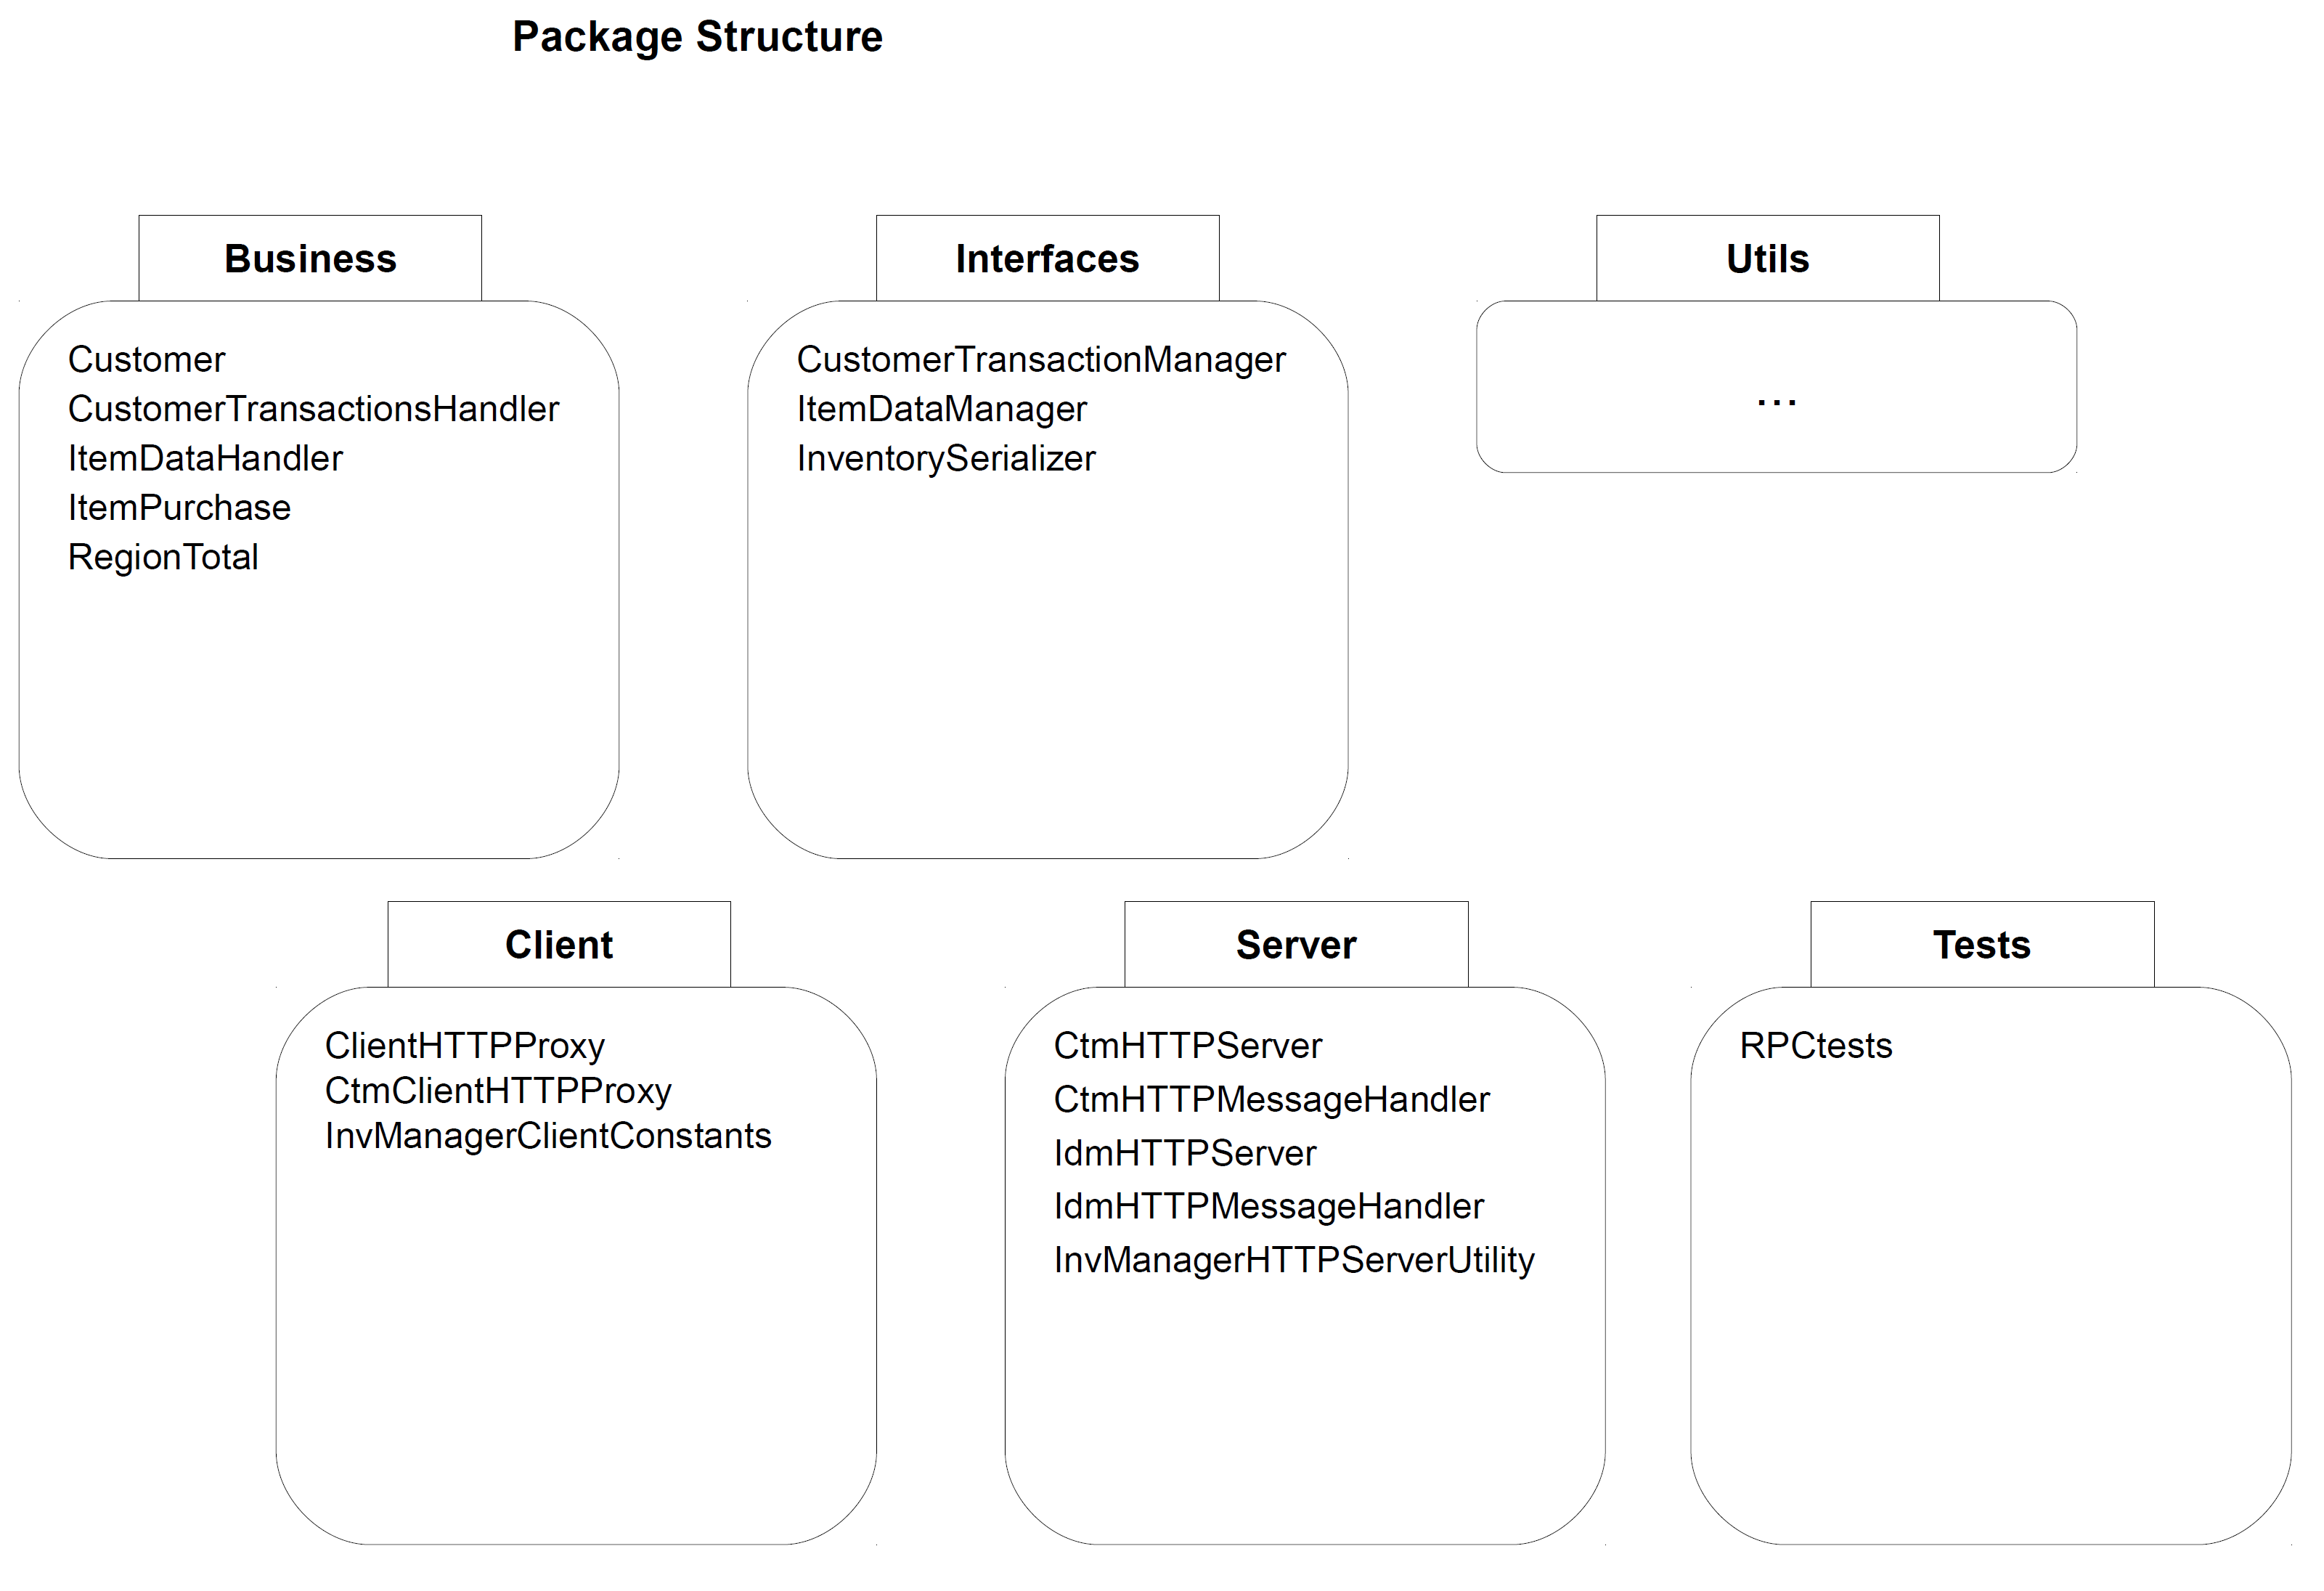
\includegraphics[width=1.1\textwidth,center]{PackageStructure.png}
\end{figure}

~\\
\textit{What RPC semantics are implemented between clients and the }\verb|CustomerTransactionManager|\textit{? What about between the} \verb|CustomerTransactionManager|\textit{ and the }\verb|ItemDataManager|\textit{? Explain.}
~\\
Regarding the RPC between clients and \verb|CustomerTransactionManager|:\\
Instead of using \verb|CustomerTransactionsHandler| as we would in a local setting, we use the class \verb|ClientHTTPProxy|, that implements the same \verb|CustomerTransactionManager| interface.\\
The \verb|ClientHTTPProxy| contains the proxy invocations that serialize the client requests and marshal them across the network.\\
~\\
Server-side, the class \verb|CtmHTTPMessageHandler| implements the naming service: it reads the keywords contained in the client messages (PROCESSORDERS, GETREGIONTOTALS, etc.) and it invokes the appropriate method to handle the request. \\
It passes the parameters to the API functions of \verb|CustomerTransactionManager|.
~\\
The class \verb|CtmHTTPServer| starts the Server for the CustomerTransactionManager layer. It listens on the DEFAULT\_PORT=8081.\\
~\\
About the RPC between the \verb|CustomerTransactionManager| layer and the \verb|ItemDataManager|s:\\
In its constructor, the intermediate layer (\verb|CustomerTransactionsHandler|) creates a number of \verb|CtmClientHTTPProxy|, that implement the \verb|ItemDataManager| interface. In the ConcurrentHashMap, each one of those has a key $i$. They listen on the port DEFAULT\_PORT + i.\\
~\\
In both cases, we implemented at-most-once RPC semantics. While some operations are idempotent (such as getTotalsForRegions) and could be repeated, we attempt to invoke a service only once.\\ 
~\\
\begin{figure}[h]
	 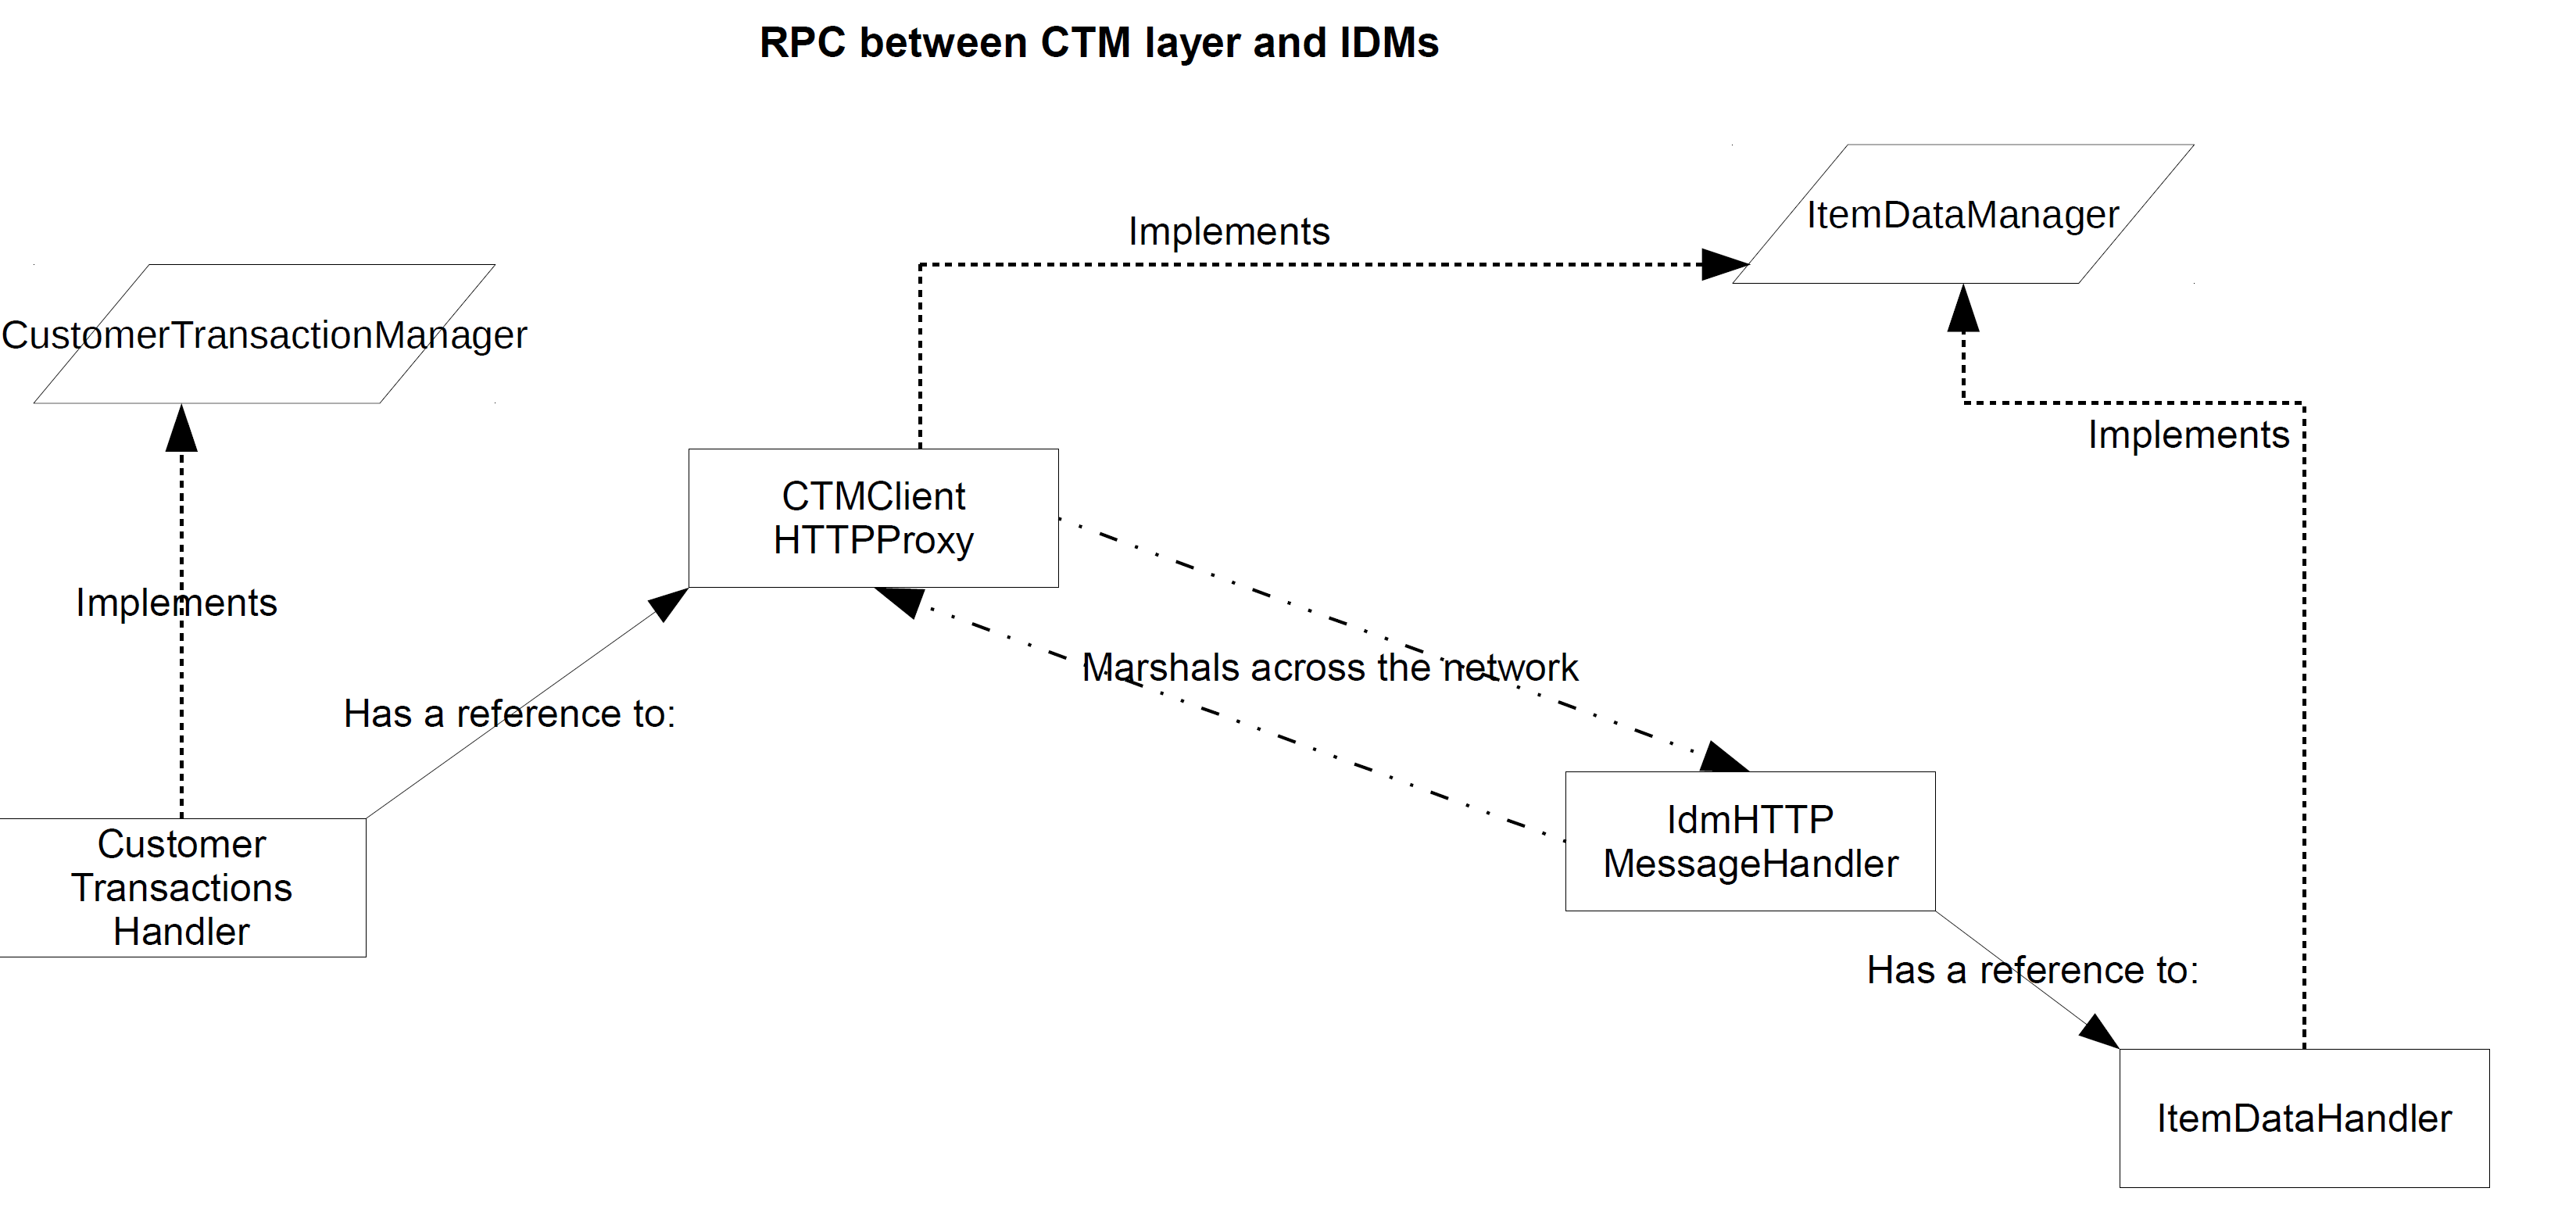
\includegraphics[width=1.0\textwidth,center]{RPC.png}
\end{figure}
~\\
\textit{How are failures of }ItemDataManager\textit{ instances contained at the}
CustomerTransactionManager\textit{? Why does your failure containment implementation turn}
\textit{out to guarantee a fail-soft design for the }CustomerTransactionManager\textit{ with respect to}
ItemDataManager\textit{ instances?}\\
~\\

\end{document}
